
\documentclass[conference]{IEEEtran}
% Some Computer Society conferences also require the compsoc mode option,
% but others use the standard conference format.
%
% If IEEEtran.cls has not been installed into the LaTeX system files,
% manually specify the path to it like:
% \documentclass[conference]{../sty/IEEEtran}





% Some very useful LaTeX packages include:
% (uncomment the ones you want to load)


% *** MISC UTILITY PACKAGES ***
%
%\usepackage{ifpdf}
% Heiko Oberdiek's ifpdf.sty is very useful if you need conditional
% compilation based on whether the output is pdf or dvi.
% usage:
% \ifpdf
%   % pdf code
% \else
%   % dvi code
% \fi
% The latest version of ifpdf.sty can be obtained from:
% http://www.ctan.org/pkg/ifpdf
% Also, note that IEEEtran.cls V1.7 and later provides a builtin
% \ifCLASSINFOpdf conditional that works the same way.
% When switching from latex to pdflatex and vice-versa, the compiler may
% have to be run twice to clear warning/error messages.






% *** CITATION PACKAGES ***
%
%\usepackage{cite}
% cite.sty was written by Donald Arseneau
% V1.6 and later of IEEEtran pre-defines the format of the cite.sty package
% \cite{} output to follow that of the IEEE. Loading the cite package will
% result in citation numbers being automatically sorted and properly
% "compressed/ranged". e.g., [1], [9], [2], [7], [5], [6] without using
% cite.sty will become [1], [2], [5]--[7], [9] using cite.sty. cite.sty's
% \cite will automatically add leading space, if needed. Use cite.sty's
% noadjust option (cite.sty V3.8 and later) if you want to turn this off
% such as if a citation ever needs to be enclosed in parenthesis.
% cite.sty is already installed on most LaTeX systems. Be sure and use
% version 5.0 (2009-03-20) and later if using hyperref.sty.
% The latest version can be obtained at:
% http://www.ctan.org/pkg/cite
% The documentation is contained in the cite.sty file itself.


\usepackage{graphicx}      % include this line if your document contains figures
%\usepackage{natbib}        % required for bibliography
\usepackage[danish,swedish,english]{babel}
%\usepackage[utf8]{inputenc}
\usepackage{url}
%\usepackage{style}
%\usepackage{float}
\usepackage{biblatex} %Imports biblatex package
%\addbibresource{mendeley.bib} %Import the bibliography file
\addbibresource{local.bib} 
%\addbibresource{springerbook_enery_analysis.bib} 


\usepackage{csquotes}
%\usepackage[sort]{natbib}
%\usepackage[sort,nocompress]{cite}
\begin{document}


\title{Smart Campus data platform and analysis \\
 \large potential for corporation with small scale Enterprises}

\author{\IEEEauthorblockN{\underline{Ole Schultz}\IEEEauthorrefmark{1},
Tomasz Blaszczyk\IEEEauthorrefmark{1},
Hakan Yurdakul Pedersen Ms. Stud. \IEEEauthorrefmark{2} and
Abdirazak Mohamud Yusuf Ms. Stud.\IEEEauthorrefmark{2}}
\IEEEauthorblockA{\IEEEauthorrefmark{1}DTU Diplom, Section for Informatics,
Center for Bachelor of Engineering Studies \\ E-mails: \underline{osch@dtu.dk},  tomb@dtu.dk}
\IEEEauthorblockA{\IEEEauthorrefmark{2} DTU, Computer Science\\
E-mails: \texttt{hakan552\_5@hotmail.com},  \texttt{Abdirazak3@hotmail.com}}}
\maketitle

\section{Introduction}
Logging  data as energy on sub-levels, indoor climate and weather can be the foundation for changing the daily process of operating buildings and processes more sustainable. Building management system samples a lot of data, but these are proprietary and access is not possible for students and researchers. At the same time we are partner in Sustainable Production in WP4\footnote{funded project by The Danish Industry Foundation}. Therefore the Campus facilities is equipped with low-cost IoT sensors. Here and at the conference we address these questions: How to utilize the energy data energy and indoor climate data in a Big Data analysis platform for improving a sustainable Campus?  How to get students involved? How can the small scale enterprises be involved together with students?

\section{Smart building data platform}
Studies show awareness of energy consumption in private homes\cite{Ali2013VisualizationHomes} and office buildings\cite{Katzeff2013ExploringConsumption}can be increased by logging, analyzing and visualizing data.\par Right know we are logging data from: Parking smart light, electrical meters, weather station, indoor climate meters. At the conference we present the platform and examples on non intrusive data loggers, some examples on analysis which can be done by zeppelin notebook\cite{zep}\cite{BigWipro1}\cite{DubyREPRODUCIBLENOTEBOOK1} 


\begin{figure}[ht]


%\centering
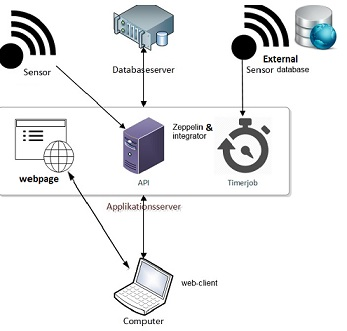
\includegraphics[scale=0.7]{datasamlings_platform2.jpg}
\centering
\caption{The data analysis domain model}
\label{fig:univerise}
\end{figure}

\par{Found in figure 1 upper right hand-corner are external cloud services with internet connected sensors : thingspeak.com, ic-meter, and an cloud server like thingspeak. Data from theses are then by timer-jobs aggregated into a common mysql-database from where the Zeppelin notebook can access data by ex. scripts as R, Python.}\par
Last semester, three Bachelor of Eng. students\IEEEauthorrefmark{2} \cite{datasamling}  configured the platform and  developed the back-end and front-end  and the sensor databases as well. The sensors were developed by\IEEEauthorrefmark{1}. 


\section{Perspectives}
This work and platform has a lot of potential and purposes corporation with the industry and do CDIO\footnote{Conceive Design Implement and Operate}-projects.The platform fits well with the monitoring and check in energy management in ISO 150001 described in \cite{EnergyIndustries1}. It can inspire for the students and the small and medium scale industry to cooperate. Students can work on real data in statistic and in the Big data 62527 courses. Another purpose, to use the data in future research on dynamics-abnormality in different parts of the building\cite{Oh2016}. Projects about visualization of data for nudging studies\cite{Ali2013VisualizationHomes}.

\printbibliography[title={References}]
\bibliographystyle{style}   % (uses file "unsrt.bst")

\end{document}
